\chapter{Interpretability}

\section{Importance of Interpretability}
Interpretability refers to the capability to explain and understand how a model arrives at its predictions or decisions. Regression models and decision trees are simple to understand and thus very popular in the banking industry. In contrary, more advanced machine learning models show a black box nature, their model logic and output are difficult to explain. Machine learning models' complex structure have advantages and disadvantages. While they can detect non-linear relationships and correlations, and may show improved accuracy or efficiency, they are prone to overfitting and lack explainability. Their black box nature stems from the model's numerous transformation of input variables, as well as their optimization process. 

\subsection{Regulatory and legal requirements}

Interpretability enables compliance with regulations and consumer protection laws such as the Capital Requirements Regulation (CRR) and General Data Protection Regulation (GDPR). Data protection principles such as purpose limitation, data minimisation and limitation on automated decisions are evident obstacles for complex AI models. In the CRR (Capital Requirements Regulation, Article 144(1)(a)), a requirement of the PD model development is stated as:

\begin{quote}

(a) the institution's rating systems provide for a meaningful assessment of obligor and transaction characteristics, a meaningful differentiation of risk and accurate and consistent quantitative estimates of risk;

\end{quote}

Regulations therefore require model developers and users to provide explanations for credit-related decisions to their customers. Modellers, internal and external audit are obligated to validate the model structure and their result, whether the model aligns with domain knowledge and expectations. Interpretability helps identify potential biases, data issues, or model limitations. Additionally, a model, which is unexplainable but is used in production, increases operational risk due to the difficulty to assess possible consequences (bias, fariness) and if the result was correctly calculated or contains a system error. To avoid the limitation of regulation requirements and consumer protection laws, machine learning models can be employed in areas, where the model structure and output are not of the highest priority, such as collection process or fraud detection. 

\subsection{Data Management}
Before the development or deployment of machine learning models, a sound data management process has to be established. The training data must be unbiased and accurately reflect the population the model will be deployed on, meaning that minority groups should not be over- or underrepresented. If the data used during the training phase or in production are not corrected and validated, this can lead to unexpected results or to a biased model. Machine learning algorithms are able to amplify the errors, as a popular saying goes "Garbage In - Garbage Out". 

\section{Methods for Interpretability Analysis}
Techniques to asses the interpretability of advanced models are also called model-agnostic explainability methods. They are algorithm independent, usually applied after model development and applied on global or local level, which means on dataset or data observation level respectively. Depending on which aspect should be analysed, the techniques can be allocated into  
five categories: feature importance, input variable impact, specific prediction analysis, output analysis and robustness check.

\subsection{Feature Importance}
Feature importance measures the contribution of each variable in a predictive model to the overall model performance. If the performance drops significantly while changing the value of a variable while holding other risk factors constant implies the importance of that feature. Relative feature importance compares the importance of features relative to each other w, which helps prioritize features based on their impact on the model's predictions. The ranges of each variable has to be normalized to the same scale, which allows a direct comparison of the impact.

\begin{figure}[H]
	\centering
	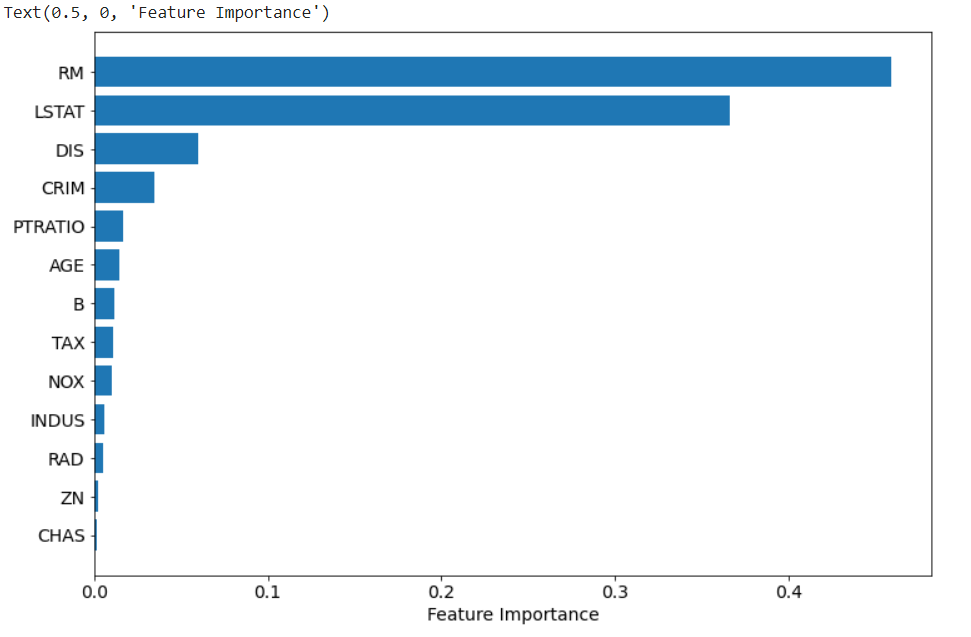
\includegraphics[width=0.625\textwidth]{./IN__featureimp.png}
    \caption{Feature Importance}
    \label{fig:in_featureimp}
\end{figure}

\subsection{Input variable impact}
Techniques to analyse the impact of different variables are Partial Dependence Plots (PDP), Individual Conditional Expectation (ICE) and saliency maps. An illustration is visible in Fig. \ref{fig:in_pdp} - \ref{fig:in_salmaps}. PDP visualises the relationship between a specific feature and the model's predictions while holding other variables constant. PDPs provide insights into the direction and magnitude of the feature's effect on default probability. ICE is an extension of PDP, where it illustrates how predictions change for an individual data point as a specific feature varies. Saliency maps highlight regions in the feature map, which contributes to the prediction. 

\begin{figure}[H]
\begin{minipage}{.5\textwidth}
	\centering
	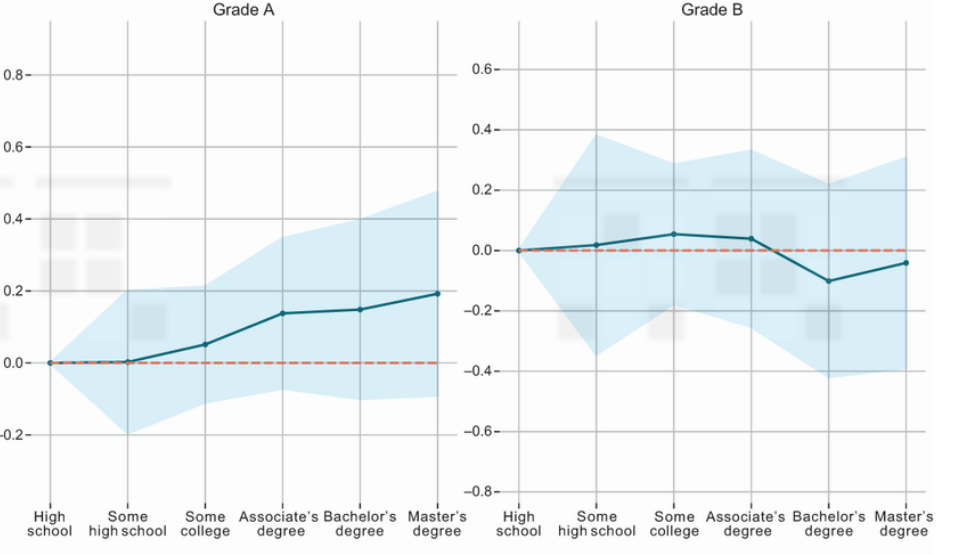
\includegraphics[width=0.9\textwidth]{./IN__PDP.png}
    \caption{Partial Dependence Plots}
    \label{fig:in_pdp}
\end{minipage}%
\begin{minipage}{.5\textwidth}
	\centering
	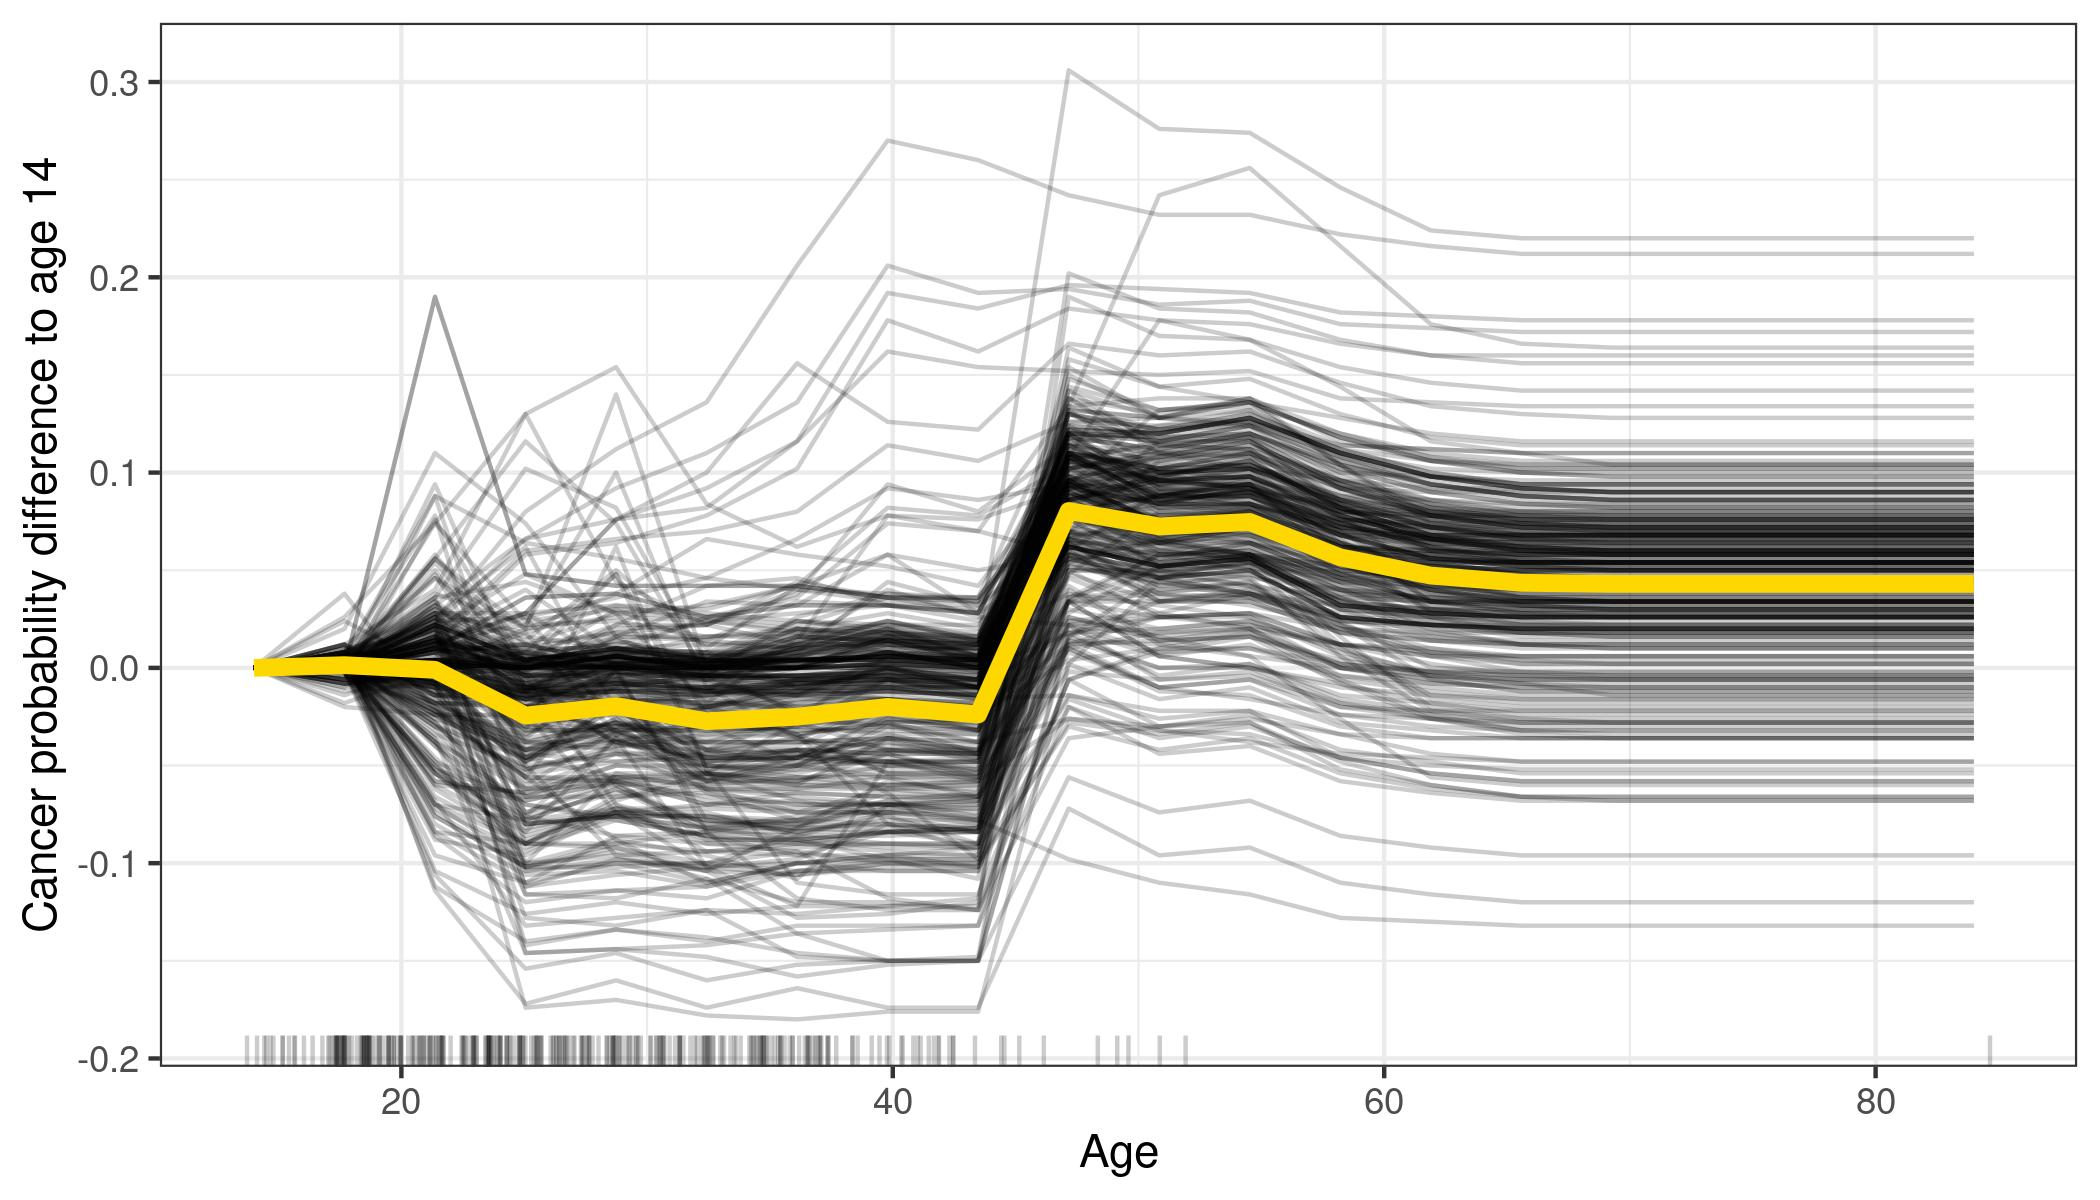
\includegraphics[width=0.9\textwidth]{./IN__ice.jpeg}
    \caption{Individual Conditional Expectation}
    \label{fig:in_ice}
\end{minipage}
\end{figure}

\begin{figure}[H]
	\centering
	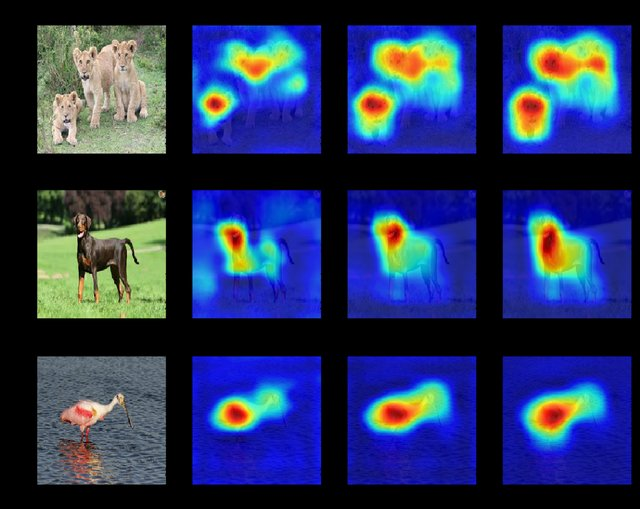
\includegraphics[width=0.625\textwidth]{./IN__saliencymaps.jpg}
    \caption{Saliency maps}
    \label{fig:in_salmaps}
\end{figure}

\subsection{Specific prediction analysis}
To interpret specific predictions, Local Interpretable Model-Agnostic Explanations (LIME, Fig. \ref{fig:in_lime}) and Local rule-based explanations can be utilized. For the LIME process, a local interpretable surrogate model is estimated. A small sample with similar variable values is selected and used to create a sparse linear regression model while using the predictions of the machine learning models as target. Similarly, the Local rule-based explanations method builds a set of decision rules as a surrogate model instead. 

\begin{figure}[H]
	\centering
	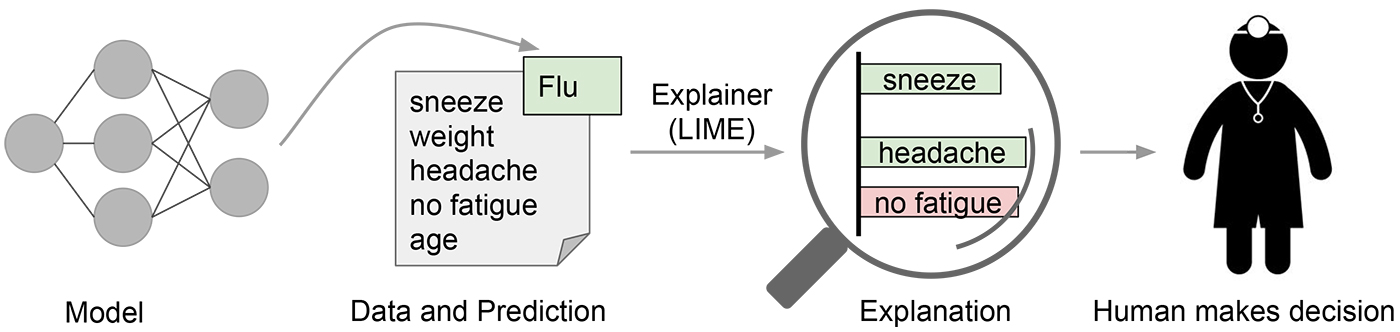
\includegraphics[width=0.625\textwidth]{./IN__lime.jpg}
    \caption{Local Interpretable Model-Agnostic Explanations}
    \label{fig:in_lime}
\end{figure}

\subsection{Output analysis and robustness check}
During Counterfactual analysis the feature values are slowly changed to assess, which total changes are necessary to receive a specific prediction. Adversial testing is performed to analyse how the machine learning model reacts to adversial attacks. Those are input data deliberately selected with the goal of causing misclassification or incorrect output. Internal layers of Deep Neural Networks can be computed to detect adversial data to respond accordingly. Alternatively, adversial data can be incorporated in the development sample to include them in the training phase. 

During the sensitivity test, data with value ranges not captured by the training sample are used to analyse the model predictions and their performance. 